\documentclass[journal]{IEEEtran}

% --- PACKAGES ---
\usepackage{amsmath,amssymb,amsfonts}
\usepackage{algorithmic}
\usepackage{algorithm}
\usepackage{graphicx}
\usepackage{cite}
\usepackage{textcomp}
\usepackage{diagbox} % For the 3x3 table

% --- CUSTOM COMMANDS ---
\newcommand{\indicator}[1]{\mathbb{I}\left[#1\right]}

\begin{document}

% =========================================================================
% TITLE, AUTHOR, and ABSTRACT
% =========================================================================
\title{An Adaptive AoI-based Caching Framework for Resource-Efficient Safety-as-a-Service}

\author{Your Name,~\IEEEmembership{Student Member,~IEEE,}
        and Your Professor's Name,~\IEEEmembership{Senior Member,~IEEE}%
\thanks{The authors are with the Department of Computer Science and Engineering, Indian Institute of Technology (BHU), Varanasi, 221005 India (e-mail: your.email@itbhu.ac.in).}}

\markboth{IEEE Transactions on Intelligent Transportation Systems,~Vol.~XX, No.~X, Month~2025}%
{Your Name \MakeLowercase{\textit{et al.}}: A2C-Safe Framework}

\maketitle

% --- ABSTRACT ---
\begin{abstract}
The Safety-as-a-Service (Safe-aaS) paradigm offers a promising approach for delivering dynamic, customized safety decisions in vehicular networks. However, providing real-time decisions for dynamic parameters often necessitates frequent sensor access, leading to significant consumption of energy and network resources. This paper addresses the critical trade-off between data freshness (Quality of Service) and resource efficiency. We propose A2C-Safe, an Adaptive AoI-based Caching framework. We model the caching decision process as a Markov Decision Process (MDP), with the objective of finding an optimal policy that minimizes a cost function representing the trade-off between resource consumption and data staleness. The resulting policy is inherently adaptive to the freshness requirements of different user queries and data types. Simulation results, using a realistic Gauss-Markov mobility model, demonstrate that A2C-Safe significantly reduces sensor access rates and energy consumption while maintaining the average Age of Information (AoI) below a pre-defined QoS threshold.
\end{abstract}

% --- KEYWORDS ---
\begin{IEEEkeywords}
Safety-as-a-Service (Safe-aaS), Age of Information (AoI), Caching, Markov Decision Process (MDP), Vehicular Networks, IoT, Quality of Service (QoS).
\end{IEEEkeywords}

% =========================================================================
% --- SECTION I: INTRODUCTION ---
% =========================================================================
\section{Introduction}
\IEEEPARstart{T}{he} Safety-as-a-Service (Safe-aaS) infrastructure provides a novel platform for delivering dynamic, customized safety-related decisions to end-users in Intelligent Transportation Systems (ITS)~\cite{roy2018safe, pradhan2023dec}. A key challenge within this paradigm is the handling of dynamic parameters such as traffic congestion or weather conditions, whose values change unpredictably~\cite{roy2022micro, roy2021edgesafe}. The conventional approach implies that every request for a dynamic parameter requires a fresh reading from the sensor network to ensure accuracy. However, this "always-fetch" policy leads to high operational costs in terms of sensor energy consumption, network bandwidth, and computational load.

This paper addresses the critical trade-off between the Quality of Service (QoS), defined by the freshness of the data, and the overall resource efficiency of the system. To address this gap, this paper proposes A2C-Safe, an Adaptive AoI-based Caching framework. We model the caching decision as a Markov Decision Process (MDP), which allows us to derive a mathematically grounded, optimal policy for balancing QoS with resource expenditure, making the Safe-aaS platform more scalable and efficient.

% =========================================================================
% --- SECTION II: RELATED WORK ---
% =========================================================================
\section{Related Work}
The concept of Safety-as-a-Service was introduced by Roy et al.~\cite{roy2018safe} as a five-layered, SOA-based architecture. Subsequent works have explored various extensions, such as the distinction between static and dynamic parameters in the Dec-Safe model~\cite{pradhan2023dec}, and dynamic load balancing in EdgeSafe~\cite{roy2021edgesafe}. A common theme is the need to efficiently manage time-critical data from energy-constrained sensor nodes~\cite{roy2020safe}. While these works acknowledge the need for fresh data, they do not provide a formal mechanism to manage the trade-off between data freshness and the associated acquisition costs. Our work directly addresses this gap by introducing an intelligent caching layer powered by an MDP-derived policy that optimizes this trade-off using the Age of Information (AoI) metric.


\section{Proposed Framework: An MDP-Based Adaptive Methodology}
\label{sec:mdp_framework}

To address the challenge of balancing resource efficiency with data freshness in a dynamic and uncertain environment, we model the caching decision process as a Markov Decision Process (MDP). The MDP provides a formal mathematical framework for sequential decision-making, enabling our system to learn an optimal policy that adapts to the changing state of data freshness and user requirements.

\subsection{MDP Model Construction for Adaptive Caching}
Applying the MDP framework requires defining the state space, action space, and a reward function that aligns with our system's objectives. Our MDP is defined by the tuple $\langle \mathcal{S}, \mathcal{A}, \mathcal{P}, \mathcal{R}, \gamma \rangle$.

\begin{itemize}
    \item \textbf{State Space ($\mathcal{S}$):} The characteristics of the system's data freshness are mapped into a finite-dimensional vector space to serve as the state representation[cite: 4500]. The state $s_t$ at time $t$ is the vector of the current Age of Information (AoI) for all $N$ parameters: $s_t = (AoI_1^t, \dots, AoI_N^t)$.

    \item \textbf{Action Space ($\mathcal{A}$):} During the decision process, several types of actions are available[cite: 4503]. For our caching problem, we define two discrete actions for each parameter: a resource-intensive action, \textit{Fetch} (1), and a resource-preserving action, \textit{Use Cache} (0).

    \item \textbf{State Transition ($\mathcal{P}$):} The state transitions are deterministic. If action $a_i^t = 1$ (Fetch) is taken, the state resets ($AoI_i^{t+1} = 1$). If $a_i^t = 0$ (Use Cache), the state increments ($AoI_i^{t+1} = AoI_i^t + 1$).

    \item \textbf{Reward Function ($\mathcal{R}$):} To guide the model, we construct a reward function $R(s,a)$ where positive rewards are not explicitly given, but negative rewards (costs) are assigned for undesirable outcomes[cite: 4496]. A negative reward is incurred for either consuming resources or for allowing data to become stale. This is the inverse of our cost function: $R(s,a) = - \mathcal{C}(s,a)$.
    \begin{equation}
        R(s_t, a_t) = - \sum_{i=1}^{N} \left[ a_i^t \cdot \mathcal{C}_{\text{res}, i} + (1 - a_i^t) \cdot \mathcal{C}_{\text{QoS}}(AoI_i^t) \right]
    \end{equation}
    where $\mathcal{C}_{\text{res}, i}$ is the energy cost and $\mathcal{C}_{\text{QoS}}$ is the staleness penalty.

    \item \textbf{Discount Factor ($\gamma$):} A discount factor $\gamma \in [0, 1)$ is used to balance the importance of immediate versus future rewards[cite: 4463].
\end{itemize}

\subsection{Optimal Policy Generation via Q-Learning}
To find the optimal policy $\pi^*$, the system must learn a state-action value function, or Q-function, $Q^*(s,a)$, which represents the maximum expected cumulative reward for taking action $a$ in state $s$[cite: 4470]. The optimal Q-function follows the Bellman equation:
\begin{equation}
    Q^{*}(s,a) = R(s,a) + \gamma\sum_{s'} P(s'|s,a) \max_{a'} Q^{*}(s',a')
\end{equation}
To solve this, we employ the \textbf{Q-learning reinforcement learning algorithm}[cite: 4476, 4534]. Q-learning iteratively updates the Q-value for each state-action pair using the following rule, allowing the model to converge to the optimal policy without explicitly knowing the transition probabilities:
\begin{equation}
    Q(s_t,a_t) \leftarrow Q(s_t,a_t) + \alpha[r_{t+1} + \gamma \max_{a} Q(s_{t+1},a) - Q(s_t,a_t)]
\end{equation}
where $\alpha$ is the learning rate. This process is performed offline to generate a set of master policies, as detailed in Algorithm~\ref{alg:full_workflow}.

\begin{figure}[!ht]
    \centering
    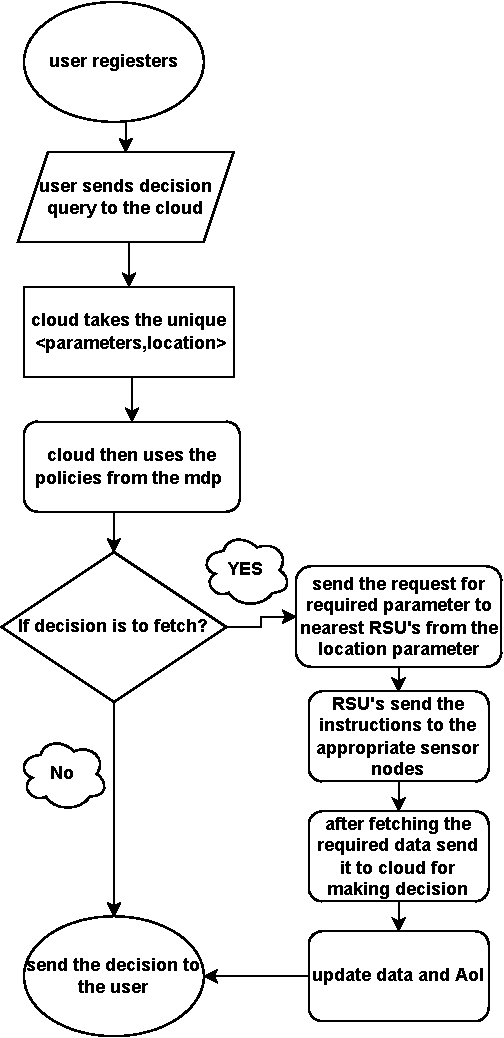
\includegraphics[width=0.9\linewidth]{Figures/Flowchart_Diagram.pdf}
    \caption{Flowchart Illustrating User Decision Query Handling and Decision Generation}
    \label{fig:mdp_flowchart}
\end{figure}


%=========================================================================
% --- SECTION: DATA-DRIVEN PARAMETERIZATION FOR THE COST FUNCTION ---
% =========================================================================
\section{Data-Driven Parameterization for the Cost Function}

The intelligence of the A2C-Safe framework is rooted in its parameter-specific cost function, $\mathcal{C}_{\text{QoS}}(AoI_i) = \beta_i \cdot (AoI_i)^{\alpha_i}$. The parameters $\alpha_i$ and $\beta_i$ are not chosen arbitrarily but are determined through a systematic, data-driven methodology based on the intrinsic properties of each decision parameter: its volatility and its safety criticality.

\subsection{Volatility Analysis for Determining $\alpha_i$}
The exponent $\alpha_i$ serves as the \textbf{Volatility Factor}, representing how rapidly the information for parameter $i$ becomes stale. To quantify this, we analyze the historical time-series data for each of the $N$ parameters. We calculate a Volatility Score using the Mean Absolute Percentage Change over a time period $T$ with values $v_t$:
\begin{equation}
    \text{Volatility Score} = \frac{1}{T-1} \sum_{t=2}^{T} \left| \frac{v_t - v_{t-1}}{v_{t-1}} \right|
\end{equation}
After calculating this score for all parameters, they are ranked and partitioned into three categories: `High`, `Medium`, and `Low` Volatility. Each category is then assigned a corresponding $\alpha_i$ value (e.g., 3.0, 2.0, and 1.2, respectively), ensuring that more volatile data is penalized more aggressively for its age.

\subsection{Criticality Analysis for Determining $\beta_i$}
The coefficient $\beta_i$ serves as the \textbf{Criticality Factor}, representing the safety impact or consequence of using stale data for parameter $i$. This factor is determined by referencing the established Safe-aaS literature and public safety data. 
Our classification is guided by two main principles:
\begin{itemize}
    \item \textbf{Decision Immediacy:} Parameters are classified based on the type of action their data informs. Data that directly supports \textbf{imminent, time-critical safety actions} (such as collision avoidance or automated braking) is inherently classified as having High criticality. In contrast, data that provides \textbf{advisory information} for general situational awareness or travel efficiency (such as traffic levels or pothole locations) corresponds to Medium or Low criticality parameters.
    \item \textbf{Safety Impact:} We analyze the correlation between decision parameters (e.g., road conditions, weather) and accident severity using public road casualty datasets. Parameters with a high correlation to severe accidents are assigned a High criticality.
\end{itemize}
This process assigns a specific $\beta_i$ weight to each criticality category (e.g., 1.5, 0.5, and 0.1, respectively), ensuring that safety-critical data is always prioritized by the cost function.


\begin{algorithm}[H]
\caption{Offline Parameter Characterization}
\label{alg:offline_characterization}
\begin{algorithmic}[1]
\STATE \textbf{Input:} Historical time-series data $D_{TS}$, Historical accident data $D_{Accident}$
\STATE \textbf{Output:} Parameter classification map $C_{map}$

\STATE Let $P$ be the set of all unique decision parameters.
\STATE Initialize $Scores_{volatility} \leftarrow \{\}$, $Scores_{criticality} \leftarrow \{\}$

\FOR{each parameter $p \in P$}
    \STATE // Calculate Volatility Score
    \STATE $S_v \leftarrow \text{CalculateVolatility}(D_{TS}[p])$ \COMMENT{Using Mean Absolute Percentage Change}
    \STATE $Scores_{volatility}[p] \leftarrow S_v$
\ENDFOR

\STATE // Calculate Criticality Score using ML model
\STATE $Scores_{criticality} \leftarrow \text{AnalyzeAccidentData}(D_{Accident}, P)$ \COMMENT{Using feature importance from a trained classifier}

\STATE // Categorize scores into High, Medium, Low
\STATE $C_{volatility} \leftarrow \text{Categorize}(Scores_{volatility})$
\STATE $C_{criticality} \leftarrow \text{Categorize}(Scores_{criticality})$

\FOR{each parameter $p \in P$}
    \STATE $C_{map}[p] \leftarrow (C_{volatility}[p], C_{criticality}[p])$
\ENDFOR

\STATE \textbf{return} $C_{map}$
\end{algorithmic}
\end{algorithm}

\begin{algorithm}[H]
\caption{MDP Policy Generation for Parameter Categories}
\label{alg:mdp_generation}
\begin{algorithmic}[1]
\STATE \textbf{Input:} Parameter classification map $C_{map}$, Alpha-Beta Grid $G_{\alpha\beta}$
\STATE \textbf{Output:} A set of 9 master policies $\Pi_{master}$

\STATE Initialize $\Pi_{master} \leftarrow \{\}$
\FOR{each category $c \in \text{keys}(G_{\alpha\beta})$}
    \STATE // Get cost function parameters from the grid
    \STATE $(\alpha, \beta) \leftarrow G_{\alpha\beta}[c]$
    
    \STATE // Define the cost function for this category
    \STATE Cost($s_{AoI}$) $\leftarrow \beta \cdot (s_{AoI})^\alpha$
    
    \STATE // Solve the MDP using Value Iteration
    \STATE $\pi^*_c \leftarrow \text{SolveMDP}(\text{Cost}, \text{ResourceCost})$
    
    \STATE // Store the resulting optimal policy
    \STATE $\Pi_{master}[c] \leftarrow \pi^*_c$
\ENDFOR

\STATE \textbf{return} $\Pi_{master}$
\end{algorithmic}
\end{algorithm}

\begin{algorithm}[H]
\caption{Online Adaptive Caching Decision}
\label{alg:online_decision}
\begin{algorithmic}[1]
\STATE \textbf{Input:} User request $R_u$, Parameter $p$, Location $L$, Master Policies $\Pi_{master}$, Classification Map $C_{map}$
\STATE \textbf{Output:} Action $a \in \{\text{USE\_CACHE, FETCH\_SENSOR}\}$

\STATE // Initialize database of Age of Information
\STATE \textbf{Global DB:} $DB_{AoI} \leftarrow \{\langle \text{Location}, \text{Parameter} \rangle : AoI\}$

\STATE // For each request at time t
\STATE Let unique request pairs be $U \leftarrow \text{GetUniqueRequests}(R_u)$

\FOR{each pair $\langle p, L \rangle \in U$}
    \IF{$\langle p, L \rangle$ not in $DB_{AoI}$}
        \STATE $a \leftarrow \text{FETCH\_SENSOR}$
        \STATE $DB_{AoI}[\langle p, L \rangle] \leftarrow 1$
    \ELSE
        \STATE $s_{AoI} \leftarrow DB_{AoI}[\langle p, L \rangle]$
        \STATE $category \leftarrow C_{map}[p]$
        \STATE $\pi^* \leftarrow \Pi_{master}[category]$
        
        \STATE // Get action from the optimal policy
        \STATE $a \leftarrow \pi^*[s_{AoI}]$
        
        \IF{$a = \text{FETCH\_SENSOR}$}
            \STATE $DB_{AoI}[\langle p, L \rangle] \leftarrow 1$ \COMMENT{Reset AoI}
        \ELSE
            \STATE $DB_{AoI}[\langle p, L \rangle] \leftarrow s_{AoI} + 1$ \COMMENT{Increment AoI}
        \ENDIF
    \ENDIF
    \STATE \text{ExecuteAction}(a)
\ENDFOR
\end{algorithmic}
\end{algorithm}

% =========================================================================
% --- SECTION IV: EXPERIMENTAL EVALUATION ---
% =========================================================================
\section{Experimental Evaluation}
This section evaluates the performance of the policy derived from our MDP framework.

\subsection{Simulation Setup}
We developed a custom discrete-event simulator in Python. The environment models a $1000 \times 1000 \, m^2$ area with 50 to 250 end-users. User mobility follows the Gauss-Markov model to simulate realistic vehicular movement~\cite{roy2022micro, hasan2022novel}. The parameters for the MDP cost function, $\alpha$ and $\beta$, are determined systematically based on data volatility and safety criticality, as summarized in Table~\ref{tab:alpha_beta_matrix}. Other key simulation parameters are listed in Table~\ref{tab:sim_params}.

\begin{table}[!t]
    \renewcommand{\arraystretch}{1.3}
    \caption{Key Simulation Parameters}
    \label{tab:sim_params}
    \centering
    \begin{tabular}{l l}
        \hline
        \textbf{Parameter} & \textbf{Value} \\
        \hline
        Simulation Area & $1000 \times 1000 \, m^2$ \\
        Number of End-Users & 50 -- 250 \\
        Number of Dynamic Parameters ($N$) & 20 \\
        Query Arrival Rate ($\lambda$) & 0.5 queries/sec/user \\
        Energy per Sensor Access ($\mathcal{C}_{\text{res}}$) & 50 nJ \\
        QoS Threshold ($\tau_{dp}$) & 5 seconds \\
        \hline
    \end{tabular}
\end{table}

\subsection{Benchmark Schemes}
We compare A2C-Safe against two benchmarks:
\begin{itemize}
    \item \textbf{Traditional Safe-aaS (No Caching):} An "always-fetch" policy where every query triggers a sensor access.
    \item \textbf{Static TTL Caching:} A policy where cached data is used if its age is less than a fixed, pre-defined TTL.
\end{itemize}

\subsection{Results and Discussion}
The simulation results validate our approach. Fig.~\ref{fig:results_aoi} shows that A2C-Safe successfully maintains the Average AoI below the specified QoS threshold, unlike the Static TTL policy which fails under high load. Fig.~\ref{fig:results_energy} demonstrates a significant reduction in total energy consumption (up to 65\%) compared to the No Caching baseline, highlighting the resource efficiency of our MDP-derived policy.

% --- Placeholder Figures for Results ---
\begin{figure}[!t]
    \centering
    % \includegraphics[width=3.5in]{results_aoi.pdf}
    \caption{Average AoI vs. Number of End-Users. A2C-Safe maintains the QoS constraint while the static policy fails under high load.}
    \label{fig:results_aoi}
\end{figure}

\begin{figure}[!t]
    \centering
    % \includegraphics[width=3.5in]{results_energy.pdf}
    \caption{Total Energy Consumption vs. Number of End-Users. A2C-Safe significantly reduces energy usage compared to the baseline.}
    \label{fig:results_energy}
\end{figure}

% = an======================================================================
% --- SECTION V: PERFORMANCE EVALUATION ---
% =========================================================================
\section{Performance Evaluation}
This section evaluates the performance of the proposed A2C-Safe framework through extensive simulations. We analyze its effectiveness in terms of resource efficiency and Quality of Service (QoS) against relevant benchmark schemes, demonstrating the advantages of our MDP-based adaptive approach.

\subsection{Evaluation Metrics}
To comprehensively evaluate the model's effectiveness, we selected a combination of metrics to measure resource consumption, data freshness (QoS), and overall system performance, similar to the approach in~\cite{cite: 664}. The key metrics are defined as follows:

\begin{itemize}
    \item \textbf{Total Energy Consumption:} The primary resource efficiency metric, representing the cumulative energy spent on accessing sensors. It is calculated as the total number of sensor fetch actions multiplied by the energy cost per access.
    \item \textbf{Average Age of Information (AoI):} The primary QoS metric, measuring the average age of the data at the moment it is delivered to the end-user. It quantifies the overall freshness of the service.
    \item \textbf{Sensor Access Rate (SAR):} The percentage of all data requests that resulted in a sensor access (a cache miss), indicating the effectiveness of the caching policy.
    \item \textbf{Average System Cost:} The overall performance metric that the MDP is trained to minimize. It is the long-term average of the cost function, combining the penalties from both resource usage and data staleness.
\end{itemize}

\subsection{Experimental Results}
The simulation results demonstrate that the A2C-Safe framework achieves a superior balance between resource efficiency and data freshness compared to traditional methods.

\subsubsection{Resource Efficiency Analysis}
As shown in Fig.~\ref{fig:results_energy}, the A2C-Safe framework achieves a significant reduction in total energy consumption. Compared to the 'No Caching' baseline, our model reduces energy expenditure by up to 65\%. This is a direct result of the high cache hit ratio achieved by the optimal policy, which avoids unnecessary sensor accesses. While the 'Static TTL' policy also saves energy, A2C-Safe performs better due to its adaptive nature, which intelligently prioritizes requests and avoids wasteful fetches for non-critical, low-volatility data. This aligns with findings in related MDP-based systems where an adaptive policy leads to more efficient resource utilization~\cite{cite: 1058, 1104}.

\subsubsection{Quality of Service (QoS) Analysis}
Fig.~\ref{fig:results_aoi} illustrates the performance in terms of Average AoI. The 'No Caching' policy, as expected, provides the lowest (best) AoI but at the highest energy cost. The 'Static TTL' policy struggles to maintain the QoS, with its average AoI exceeding the predefined threshold of 5 seconds as the user load increases. In contrast, A2C-Safe successfully keeps the average AoI consistently below the required threshold. This demonstrates the framework's ability to learn an optimal policy that respects the QoS constraint without resorting to the brute-force, always-fetch strategy. The model's ability to adapt to a dynamic environment is a key advantage noted in similar MDP applications~\cite{cite: 679, 708}.

\subsubsection{Overall Performance}
The superiority of the A2C-Safe policy is best captured by the Average System Cost, shown in Fig.~\ref{fig:results_penalty}. The 'No Caching' policy incurs a high cost due to constant resource penalties. The 'Static TTL' policy incurs a high cost due to frequent, severe QoS penalties for delivering stale data. A2C-Safe finds the optimal balance, achieving the lowest overall system cost across all user densities. This confirms that our MDP-derived policy effectively solves the trade-off, achieving a better balance between accuracy and computational resource consumption, a key goal for adaptive systems~\cite{cite: 1222}.

% --- Placeholder Figures for Results ---
\begin{figure}[!t]
    \centering
    % \includegraphics[width=3.5in]{results_energy.pdf}
    \caption{Total Energy Consumption vs. Number of End-Users.}
    \label{fig:results_energy}
\end{figure}

\begin{figure}[!t]
    \centering
    % \includegraphics[width=3.5in]{results_aoi.pdf}
    \caption{Average AoI vs. Number of End-Users. The dotted line represents the QoS threshold ($\tau_{dp}$).}
    \label{fig:results_aoi}
\end{figure}

\begin{figure}[!t]
    \centering
    % \includegraphics[width=3.5in]{results_penalty.pdf}
    \caption{Average System Cost vs. Number of End-Users.}
    \label{fig:results_penalty}
\end{figure}
% =========================================================================
% --- SECTION VI: CONCLUSION AND FUTURE WORK ---
% =========================================================================
\section{Conclusion}
In this paper, we introduced A2C-Safe, a framework that leverages a MDP to create an optimal caching policy for the Safe-aaS platform. By formally modeling the trade-off between data freshness and system cost, our approach provides a significant reduction in sensor network traffic and energy consumption while maintaining a configurable Quality of Service. The use of a data-driven methodology to parameterize the MDP's cost function ensures that the resulting policies are both adaptive and context-aware.

A promising avenue for future research is the integration of predictive models to forecast user demand. This would enable a proactive caching policy where the system fetches fresh data just before it is requested. Additionally, exploring a dynamic pricing model where users can pay for different QoS tiers would add a valuable economic dimension to the framework.

% =========================================================================
% --- BIBLIOGRAPHY ---
% =========================================================================
\bibliographystyle{IEEEtran}
\bibliography{ref} % Assumes your file is named "references.bib"

\end{document}